\section{Distributed Control Approach}
\label{sec:mpc:distributed}

\subsection{Optimization Problem}

In the distributed MPC approach, the control problem is split into two smaller optimizations, each giving the optimal input for a single compressor, and each solved by a sub-controller.
The two sub-controllers are assumed to have full state information and the optimizations are set up as QPs, as in \eqref{eq:mpc:optimization-qp-formulation}. The Hessian ($H$) term of the QP is also identical. A slight modification to the linear term -- given for the centralized case in \eqref{eq:mpc:optimization-qp-terms} -- is necessary to account for the fact that the QP is solved for only part of the optimal input vector:

\begin{equation}
  \begin{split}
    H\ut{distributed} & = 2\left( \gi{weights} + \tps{\gi{prediction-matrices}}\ \gii{weights}\ \gi{prediction-matrices} \right)\\
    & = H\ut{centralized}\\
    g\ut{distributed} & = 2\left( \g{xaug} \tps{\gii{prediction-matrices}} + \g{fcurr} \tps{\giii{prediction-matrices}} - \gi{Yrefk} + \gi{Uother}\ \tps{\g{prediction-uother}} \right)\gii{weights}\ \gi{prediction-matrices}\\
    & = g\ut{centralized} + \gi{Uother}\ \tps{\g{prediction-uother}} \gii{weights}\ \gi{prediction-matrices}\\
  \end{split}
  \label{eq:mpc:distributed-qp-terms}
\end{equation}

\noindent where \g{Uother} is the optimal input at time step $k$ calculated by the other sub-controller, and \g{prediction-uother} is the prediction matrix giving the effect of the other sub-controller's inputs on the current outputs \gi{Yk}.

As stated in \eqref{eq:mpc:distributed-qp-terms} the QP is unsolvable since \g{Uother} in turn depends on the solution.
To break this circular dependency, the problem is initially solved with an estimate for \g{Uother} obtained from the previous QP solution.
The sub-controllers then exchange information about their obtained solution, updating the value of \g{Uother} and re-solving the optimization.
This procedure is repeated for a fixed number of iterations, after which the optimal solution is sent to the plant.
The iteration process may not converge for systems that have a high degree of coupling; this effect is discussed in further detail in \cite{Stewart2010}.

The algorithm used to obtain the optimal input at each time step for a distributed controller is thus as follows:

\begin{enumerate}
  \item perform estimation to obtain the current estimate of the augmented state vector (see \sect{mpc:estimation});
  \item linearize, discretize and augment non-linear model about the current state estimate and previous inputs, as described in \sect{mpc:linearization};
  \item generate the prediction matrices using \eqref{eq:mpc:augmented-state-eqs};
  \item set up the QP problems according to \eqref{eq:mpc:optimization-qp-formulation};
  \item approximate the solution from each sub-controller using the solution from the previous iteration and use it to correct the linear QP terms;
  \item iteratively solve each QP, updating the approximation of  \g{Uother} after each iteration;
  \item after a fixed number of iterations, apply the optimal input from each sub-controller at the first prediction interval to the system.
\end{enumerate}

The algorithm and the iterative solving procedure is depicted in \fig{mpc:distributed:algo}.


\newcommand{\blockheight}{0.7}
\newcommand{\blockwidth}{1.6}
\def\blockthick{3pt}
\def\flowthick{2pt}
\newcommand{\arrowtext}[1]{\large\textbf{#1}}
\begin{figure}
  \centering
  \begin{tikzpicture}
    %
    % Main nodes
    %
    \node[align=center] (observer) at (0,0) {Observer \&\\Linearization};
    \draw[line width=\blockthick, color=black] ($(observer) + (\blockwidth,\blockheight)$) rectangle ($(observer) - (\blockwidth,\blockheight)$);
    %
    \node[align=center] (qp-gen) at ($(observer) + 5*(\blockwidth,0)$) {QP Problem\\Generation};
    \draw[line width=\blockthick, color=black] ($(qp-gen) + (\blockwidth,\blockheight)$) rectangle ($(qp-gen) - (\blockwidth,\blockheight)$);
    %
    \node[align=center] (qp-solve) at ($(qp-gen) - 4*(0,\blockheight)$) {QP Solver\\\& Output};
    \draw[line width=\blockthick, color=black] ($(qp-solve) + (\blockwidth,\blockheight)$) rectangle ($(qp-solve) - (\blockwidth,\blockheight)$);
    %
    \node[align=center] (pred) at ($(observer) - 4*(0,\blockheight)$) {State\\ Prediction};
    \draw[line width=\blockthick, color=black] ($(pred) + (\blockwidth,\blockheight)$) rectangle ($(pred) - (\blockwidth,\blockheight)$);
    %

    %
    % Arrows
    %
    \draw[<-, line width=\flowthick] ($(observer) - (\blockwidth,0)$) -- ++(-\blockwidth,0) node[above right] {\arrowtext{$\vc{y}$}};
    \draw[->, line width=\flowthick] ($(observer) + (\blockwidth,0)$)  -- ($(qp-gen) - (\blockwidth,0)$);
    \draw[->, line width=\flowthick] ($(qp-gen) - (0,\blockheight)$) -- ($(qp-solve) + (0,\blockheight)$);
    \draw[->, line width=\flowthick] ($(qp-solve) - (\blockwidth,0)$) -- ($(pred) + (\blockwidth,0)$);
    \draw[->, line width=\flowthick] ($(pred) + (0,\blockheight)$) -- ($(observer) - (0,\blockheight)$);
    \draw[->, line width=\flowthick] ($0.5*(qp-solve) + 0.5*(pred)$) |- ($(pred) - 2*(0, \blockheight)$) node[left] {\arrowtext{To plant}};

    %
    % Labels
    %
    \node[above] at ($0.5*(observer) + 0.5*(qp-gen)$) {\arrowtext{\g{xaug}, \g{augsys-mats}}};
    \node[left] at ($0.5*(qp-gen) + 0.5*(qp-solve)$) {\arrowtext{QP}};
    \node[above] at ($0.5*(pred) + 0.5*(qp-solve)$) {\arrowtext{$\vc{u}$}};
    \node[right] at ($0.5*(pred) + 0.5*(observer)$) {\arrowtext{$\vc{\hat{x}}_{k|k-1}^a$}};

    %
    % Distributed
    %
    \draw[line width=1pt, dotted] ($(qp-solve) + 1.5*(\blockwidth,\blockheight)$) rectangle ($(qp-solve) - 1.5*(\blockwidth,\blockheight)$);
    \draw[->,dotted,line width=\flowthick] ($(qp-solve) - 1.5*(0, \blockheight)$) -- ($0.5*(qp-solve) + 0.5*(pred) - 5*(0,\blockheight)$) coordinate (dist);

    \draw[line width=1pt, dotted] ($(dist) - (5,0)$) rectangle ++(9,-6);
    
    \node[text width=2cm,align=center] (qp1) at ($(dist) - (1.5,1.5)$) {QP Solver 1};
    \node[text width=2cm,align=center] (qp2) at ($(dist) + (2.5,-1.5)$) {QP Solver 1};
    \node[text width=2cm,align=center] (qp3) at ($(qp1) - (0,2.5)$) {QP Solver 2};
    \node[text width=2cm,align=center] (qp4) at ($(qp2) - (0,2.5)$) {QP Solver 2};

    \draw[line width=\blockthick] ($(qp1) - (1,1)$) rectangle ($(qp1) + (1,1)$);
    \draw[line width=\blockthick] ($(qp2) - (1,1)$) rectangle ($(qp2) + (1,1)$);
    \draw[line width=\blockthick] ($(qp3) - (1,1)$) rectangle ($(qp3) + (1,1)$);
    \draw[line width=\blockthick] ($(qp4) - (1,1)$) rectangle ($(qp4) + (1,1)$);

    \draw[<-,line width=2pt] ($(qp2) + (1,0)$) -- ($(qp2) + (2,0)$) node[right] {QP1};
    \draw[<-,line width=2pt] ($(qp4) + (1,0)$) -- ($(qp4) + (2,0)$) node[right] {QP2};
    \draw[->,line width=2pt] ($(qp4) - (1,0)$) node[left] {\arrowtext{\gii{un}}} -- ($(qp1) + (1,0) + (4pt,0)$); 
    \draw[->,line width=2pt] ($(qp2) - (1,0)$) node[left] {\arrowtext{\gi{un}}} -- ($(qp3) + (1,0) + (4pt,0)$); 

    \draw[->,line width=2pt] ($(qp1) - (1,0)$) node[left] {\arrowtext{\gii{un}}} -- +(-2,-2.5);
    \draw[->,line width=2pt] ($(qp3) - (1,0)$) node[left] {\arrowtext{\gi{un}}} -- +(-2,2.5);

    \node[left] at ($0.5*(qp1) + 0.5*(qp3) - (2,0)$) {\huge $\bm{\cdots}$};

  \end{tikzpicture}
  \caption[Controller algorithm.]{Diagram of controller algorithm. Dashed rectangle shows procedure of distributed QP solver.}
  \label{fig:mpc:distributed:algo}
\end{figure}




\subsection{Stopping Criterion}
\label{sec:mpc:distributed:stopping}

The distributed optimization problem is iterative and a stopping criterion must therefore be chosen.
To maintain a relatively constant computation time, the best approach is to choose a fixed number of iterations for which the tradeoff between performance and computational complexity is optimal.
An alternate approach is to use the change in cost function as a criterion for convergence, however this leads to a variable number of iterations (and thus greater variation in the computation times) and it requires the cost function to be computed at each solver iteration -- adding a non-negligible computational cost.
\footnote{The cost function used by the QP solver (defined in \eqref{eq:mpc:optimization-qp-formulation}) is not equal to the actual cost function of the control problem (defined in \eqref{eq:mpc:cost-function-centralized}) as terms that do not depend on the optimization variable are excluded. Evaluating the cost function therefore requires \eqref{eq:mpc:cost-function-centralized} to be computed. This computation is relatively expensive since \gi{Delta}\g{Yk} must first be evaluated using the prediction matrices.}

For controllers whose performance is significantly dependent on the number of iterations, this additional cost could be justified, however the present systems' cost functions converge relatively quickly, as shown in \fig{mpc:distributed:cost-function}.
The average improvement between its value at 3 iterations and the optimal value reached is just 0.03\% for the serial, cooperative controller, for example.
The other distributed controllers show similar behavior.
Furthermore, the controllers exhibited no measurable change in performance for solver iterations greater than 3.
The number of iterations was therefore fixed at 3 for all distributed controllers.


\begin{figure}
  \centering
  % This file was created by matlab2tikz.
%
\definecolor{mycolor1}{rgb}{0.00000,0.44700,0.74100}%
\definecolor{mycolor2}{rgb}{0.85000,0.32500,0.09800}%
%
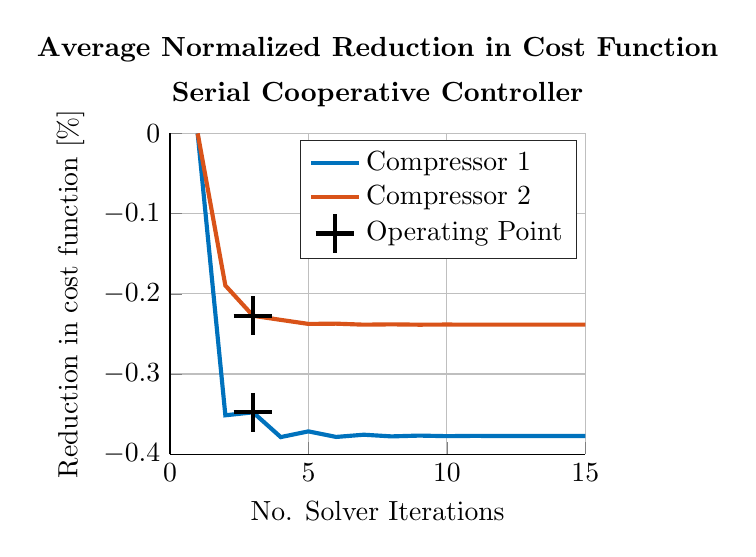
\begin{tikzpicture}

\begin{axis}[%
width=0.435\linewidth,
height=0.336\linewidth,
at={(0\linewidth,0\linewidth)},
scale only axis,
xmin=0,
xmax=15,
xlabel={No. Solver Iterations},
xmajorgrids,
ymin=-0.4,
ymax=0,
ylabel={Reduction in cost function [\%]},
ymajorgrids,
\yaxisfixedformat,
axis background/.style={fill=white},
title style={font=\bfseries,align=center},
title={Average Normalized Reduction in Cost Function\\[1ex]Serial Cooperative Controller},
axis x line*=bottom,
axis y line*=left,
legend style={legend cell align=left,align=left,draw=white!15!black}
]
\addplot [color=mycolor1,solid,line width=1.5pt]
  table[row sep=crcr]{%
1	0\\
2	-0.351501613218839\\
3	-0.347839931152752\\
4	-0.378695334349781\\
5	-0.371560054624705\\
6	-0.378510265072551\\
7	-0.375735021436657\\
8	-0.377828738041513\\
9	-0.376830921598539\\
10	-0.377530570057489\\
11	-0.377185999069046\\
12	-0.377416179102001\\
13	-0.377295424447187\\
14	-0.377375200097836\\
15	-0.377337458390244\\
16	-0.377364595958364\\
17	-0.377349227668906\\
18	-0.377360273860182\\
19	-0.377355015468009\\
20	-0.37735515497366\\
};
\addlegendentry{Compressor 1};

\addplot [color=mycolor2,solid,line width=1.5pt]
  table[row sep=crcr]{%
1	0\\
2	-0.189670745988881\\
3	-0.2274190261111\\
4	-0.232549760739897\\
5	-0.237579028892318\\
6	-0.237264216933177\\
7	-0.2385210210162\\
8	-0.238126599004626\\
9	-0.238544648969515\\
10	-0.238369635465122\\
11	-0.238521073839856\\
12	-0.23844798425613\\
13	-0.238495435705717\\
14	-0.238465167305055\\
15	-0.238485266779419\\
16	-0.238480099282162\\
17	-0.238485130829961\\
18	-0.238483669025924\\
19	-0.238485229140346\\
20	-0.238483271357933\\
};
\addlegendentry{Compressor 2};

\addplot [color=black,line width=1.5pt,mark size=7.0pt,only marks,mark=+,mark options={solid}]
  table[row sep=crcr]{%
3	-0.347839931152752\\
};
\addlegendentry{Operating Point};

\addplot [color=black,line width=1.5pt,mark size=7.0pt,only marks,mark=+,mark options={solid},forget plot]
  table[row sep=crcr]{%
3	-0.2274190261111\\
};
\end{axis}
\end{tikzpicture}%

  \caption[Average reduction in cost function as a function of the number of solver iterations.]{Average reduction in cost function as a function of the number of solver iterations for the serial, cooperative controller. Results are similar for other distributed controllers. 3 iterations were determined to be sufficient for convergence since further gains in the cost function are limited.}
  \label{fig:mpc:distributed:cost-function}
\end{figure}


\subsection{Computational Cost}

The primary advantage of distributed control over centralized control is that it allows the computational cost of the MPC controller to be reduced.
The QPs can be solved in parallel using a separate thread or even a separate device for each sub-controller.
Although the method still requires solving several QPs per sub-controller at each time step, they are smaller than the single QP solved by the centralized controller and can often be solved more efficiently.
In particular, the ``hotstart'' method implemented in the \qpoases{} QP solver can solve a QP using a previous solution as a starting point, efficiently solving series of QPs in which the Hessian and linear terms change only slightly, further reducing the computational cost of the extra iterations.

Finally, generating the prediction matrices for the sub-controllers' cost functions can be less computationally expensive than for the centralized case, if they use fewer of the outputs, since computing the prediction matrices is $\mathcal{O}(n)$ in the number of outputs used.
The computational cost could be further reduced by limiting the state information used by each sub-controller to generate its prediction matrices ($\mathcal{O}(n^3)$ in the number of states used), however this approach is not considered here.
These effects are quantified and discussed further in \sect{results:computation}.

